\section*{Dati e risultati}

\subsection*{Circuito invertente}

Il primo circuito studiato sfrutta l'opamp LM741 al fine di amplificare e sfasare di $180^\circ$ in ingresso ($V\ped{in}$). Il circuito che abbiamo realizzato è illustrato in Figura \ref{fig:amp_inv}.
Questo circuito è alimentato con una tensione costante positiva di $\SI{+15}{\volt}$ e una negativa di $\SI{-15}{\volt}$, un segnale in ingresso variabile ($V\ped{in}$) ottenuto grazie al generatore di onde.
dal momento che vogliamo che tale circuito abbia un guadagno ($G$) di circa 10 dobbiamo dimensionare il circuito. In particolare sapendo che per un circuito invertente vale la relazione:

\begin{equation}
        G\,=\,-\frac{V\ped{out}}{V\ped{in}}\,=\,-\frac{R_2}{R_1} \qquad => \qquad |R_2|\,=\,10\,|R_1|
        \label{eq:g}
\end{equation}

dove $R_1$ e $R_2$ sono le resistenze del circuito in analisi, $V\ped{in}$ il segnale in ingresso e $V\ped{out}$ il segnale in uscita. Quindi, per non avere intensità di correnti troppo elevate all'interno del circuito, abbiamo deciso di porre $R_2\,=\,\SI{100}{\kilo\ohm}$ e $R_2\,=\,\SI{10}{\kilo\ohm}$.

Fatto questo abbiamo verificato che il guadagno di tale circuito, a frequenza fissta $\nu\,=\,\SI{1}{\kilo\hertz}$, rimanesse costante al variare dell'ampiezza picco-picco in ingresso $V\ped{in}$. Pertanto sfruttando la relazione (\ref{eq:g}) abbiamo fatto la media dei valori di $G$ ricavati e abbiamo ottenuto che il guadagno del nostro circuito vale:

\begin{equation}
        G\,=\, XXX
\end{equation}

Successivamente abbiamo deciso di studiare come varia il guadagno di tale circuito al variare della frequenza di $V\ped{in}$, mantenendo costante l'ampiezza di $V\ped{in}$. Quello che abbiamo ottenuto è riportato in Figura \ref{fig:g_vs_freq}

\begin{figure}
    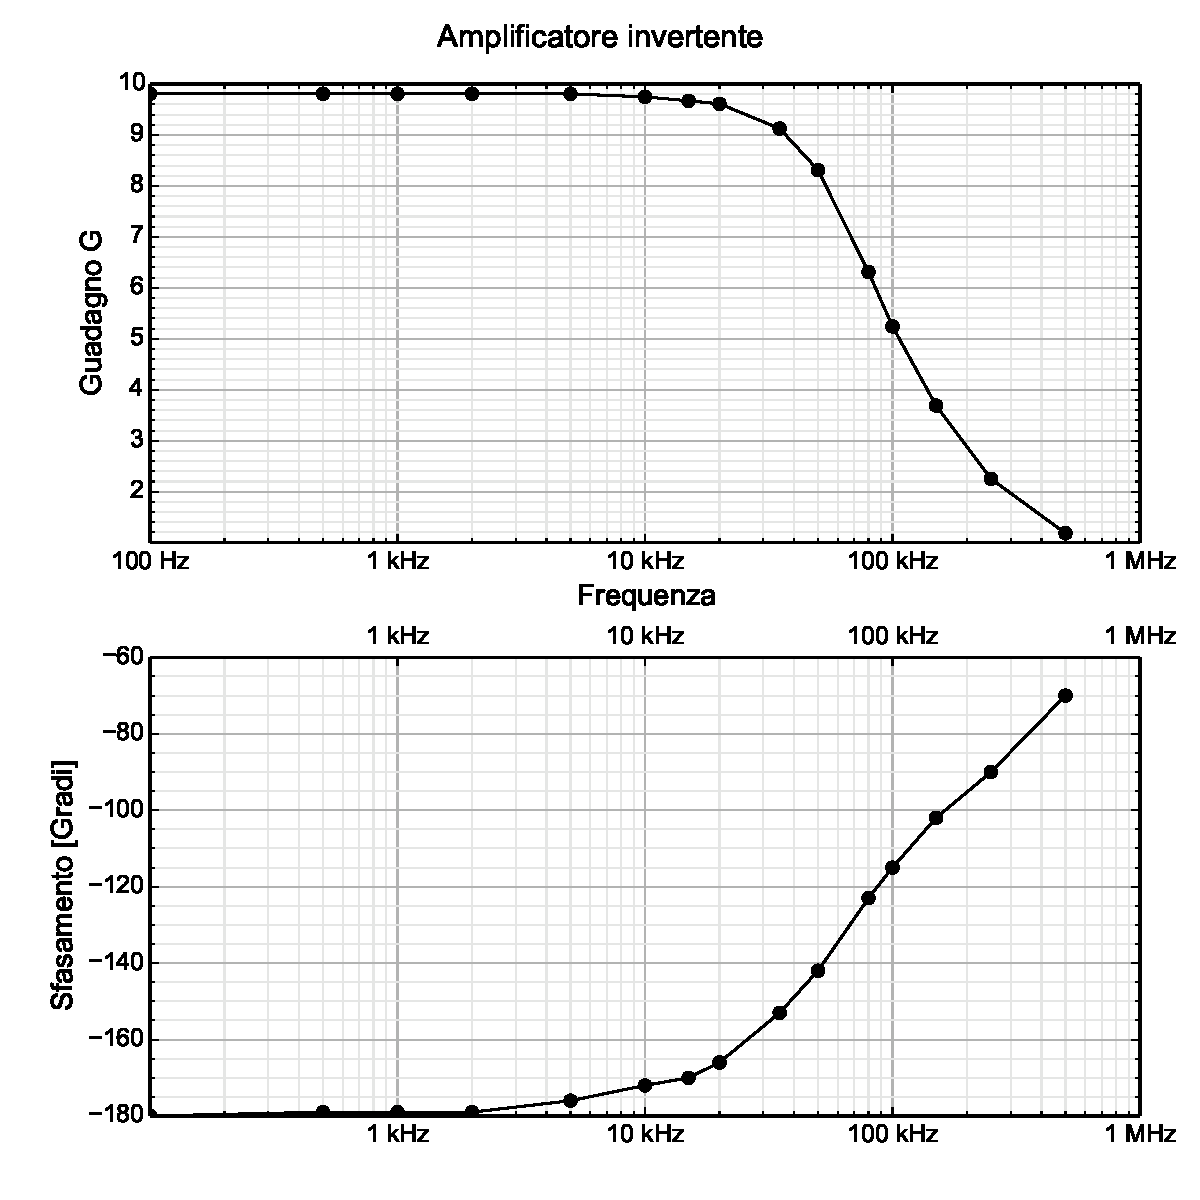
\includegraphics[width=0.75\textwidth]{amp_inv.pdf}
\end{figure}

Infine abbiamo trovato i valori di ampiezza del segnale in uscita $V\ped{out}$, a frequenza costante $\nu\,=\,\SI{1}{\kilo\hertz}$ di $V\ped{in}$, per i quali si verifica il fenomeno del clamping. Tali valori sono risultati essere:

\begin{equation}
        V\ped{out}^+\,\simeq\,\SI{14.2}{\volt} \qquad \text{e} \qquad V\ped{out}^-\,\simeq\,\SI{-13.1}{\volt}
\end{equation}



